\chapter{Le cancer de la prostate}     % numéroté
% * <larchamb@gmail.com> 2017-08-30T18:25:34.858Z:
% 
% > Le cancer de la prostate
% Ce chapitre pourrait être fusionné avec l'introduction. 
% Les section 1.1 à 1.3 devraient être assez courtes
% 
% ^ <larchamb@gmail.com> 2017-08-30T19:41:31.654Z.
\section{Incidence et mortalité}
Le cancer est classé par l’Organisation mondiale de la Santé (OMS) \cite{OMS} \nomenclature{OMS}{Organisation mondiale de la Santé} comme étant la deuxième cause de mortalité dans le monde. Les dernières statistiques de GLOBOCAN 2012 \cite{GLOBOCAN} publiées en décembre 2013 estiment à 14,1 millions, le nombre de nouveaux cas de cancer et à 8,2 millions le nombre de décès liés au cancer survenus en 2012, en comparaison respectivement à 12,7 et 7,6 millions en 2008. L’OMS souligne qu’en 2015, 8,8 millions de décès sont attribués au cancer et que, près d’un décès sur 6 dans le monde est dû au cancer. Ces chiffres interpelant peuvent s’expliquer par plusieurs facteurs, entre autres : la croissance démographique et le vieillissement de la population, une augmentation de la prévalence des facteurs de risques bien établis tels que le tabagisme, le surpoids et l'inactivité physique \cite{Torre}. Sur le plan national, la publication \enquote{statistique canadienne sur le cancer} diffusée le 20 juin 2017 \cite{StatCanada} indique que le cancer est la première cause de mortalité au Canada, soit \textasciitilde 30\% par rapport aux autres maladies. La figure \ref{FigureStatCancer1} \cite{StatCanada} illustre le taux de mortalité au Canada en 2012, pour l'ensembles des causes de décès confondus.
%
\begin{figure}%[h]
\centering
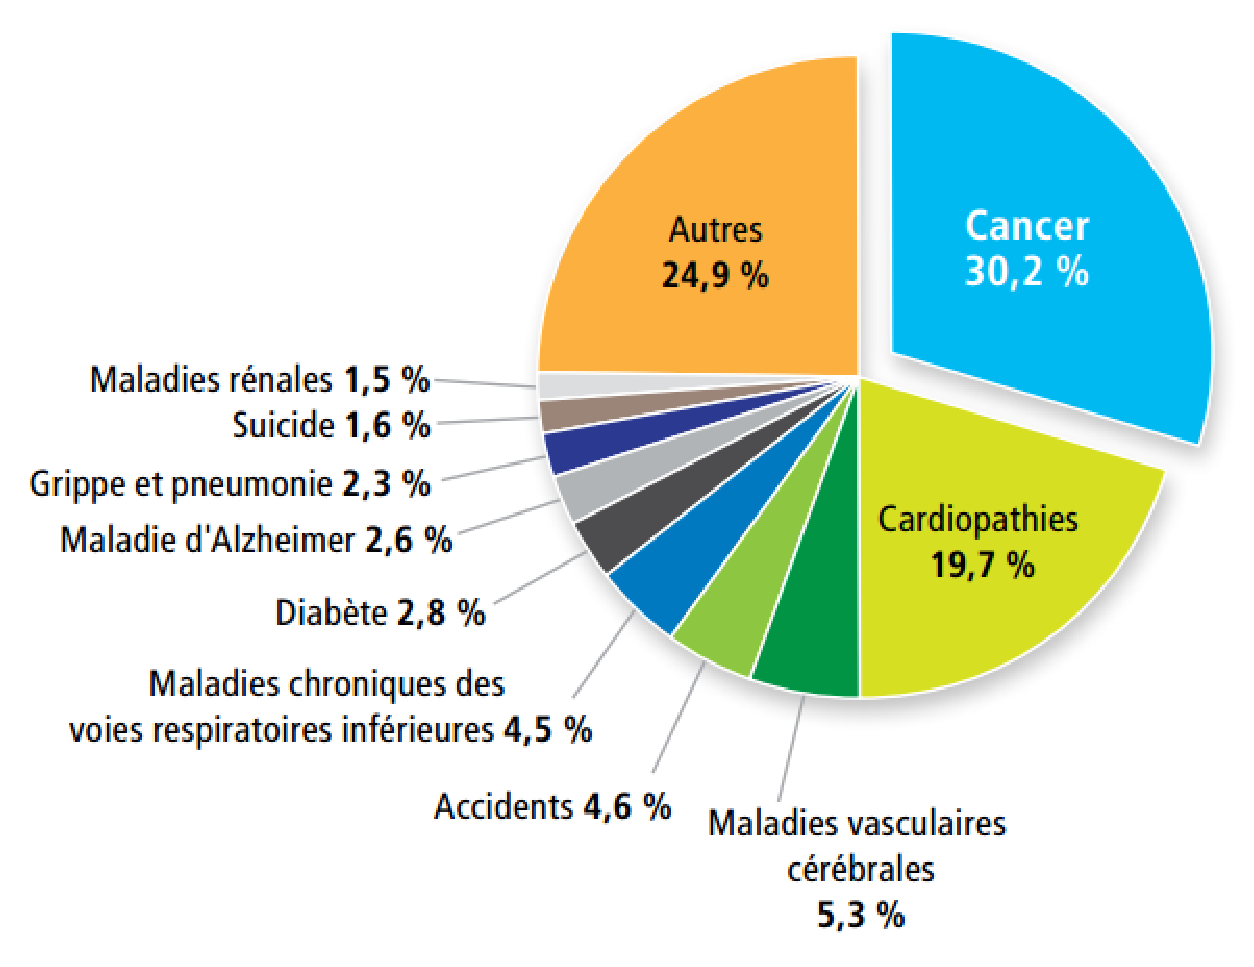
\includegraphics[width=7.3cm,height=5.5cm]{FigureStatCancer1.eps}
\caption{\label{FigureStatCancer1} Taux de mortalité au Canada en 2012, toutes causes confondues.}
\end{figure}
%
Les estimations sur l’incidence et la mortalité en 2017 sont \textasciitilde 100 000 et 42 500 nouveaux cas pour les hommes, respectivement. La tendance est similaire pour les femmes, à savoir, \textasciitilde 100 000 et 37 500, respectivement. La figure \ref{FigureStatCancer2} \cite{StatCanada} montre la répartition des années potentielles de vie perdues (APVP) \nomenclature{APVP}{Années Potentielles de Vie Perdues} dues au cancer, comparativement à d’autres causes de décès, et leurs distributions par rapport au sexe. En ce qui concerne les différents types de cancer chez l’homme, la même publication rapporte le cancer de la prostate comme ayant la plus grande incidence. La projection de nouveaux cas en 2017 pour le cancer de la prostate est 20,7\%, suivi du cancer colorectal (14.5\%) et le cancer des poumons et bronches (14\%). Les chiffres sans doute alarmants présentés ci-dessus, aussi bien sur le plan mondial que national, peuvent expliquer la grande mobilisation observée dans le monde pour le recherche sur le cancer; recherches orientées soit dans le perfectionnement des méthodes de traitements actuellement utilisés en clinique, ou dans le développement de nouvelles possibilités thérapeutiques.
%
\begin{figure}[h]
\centering
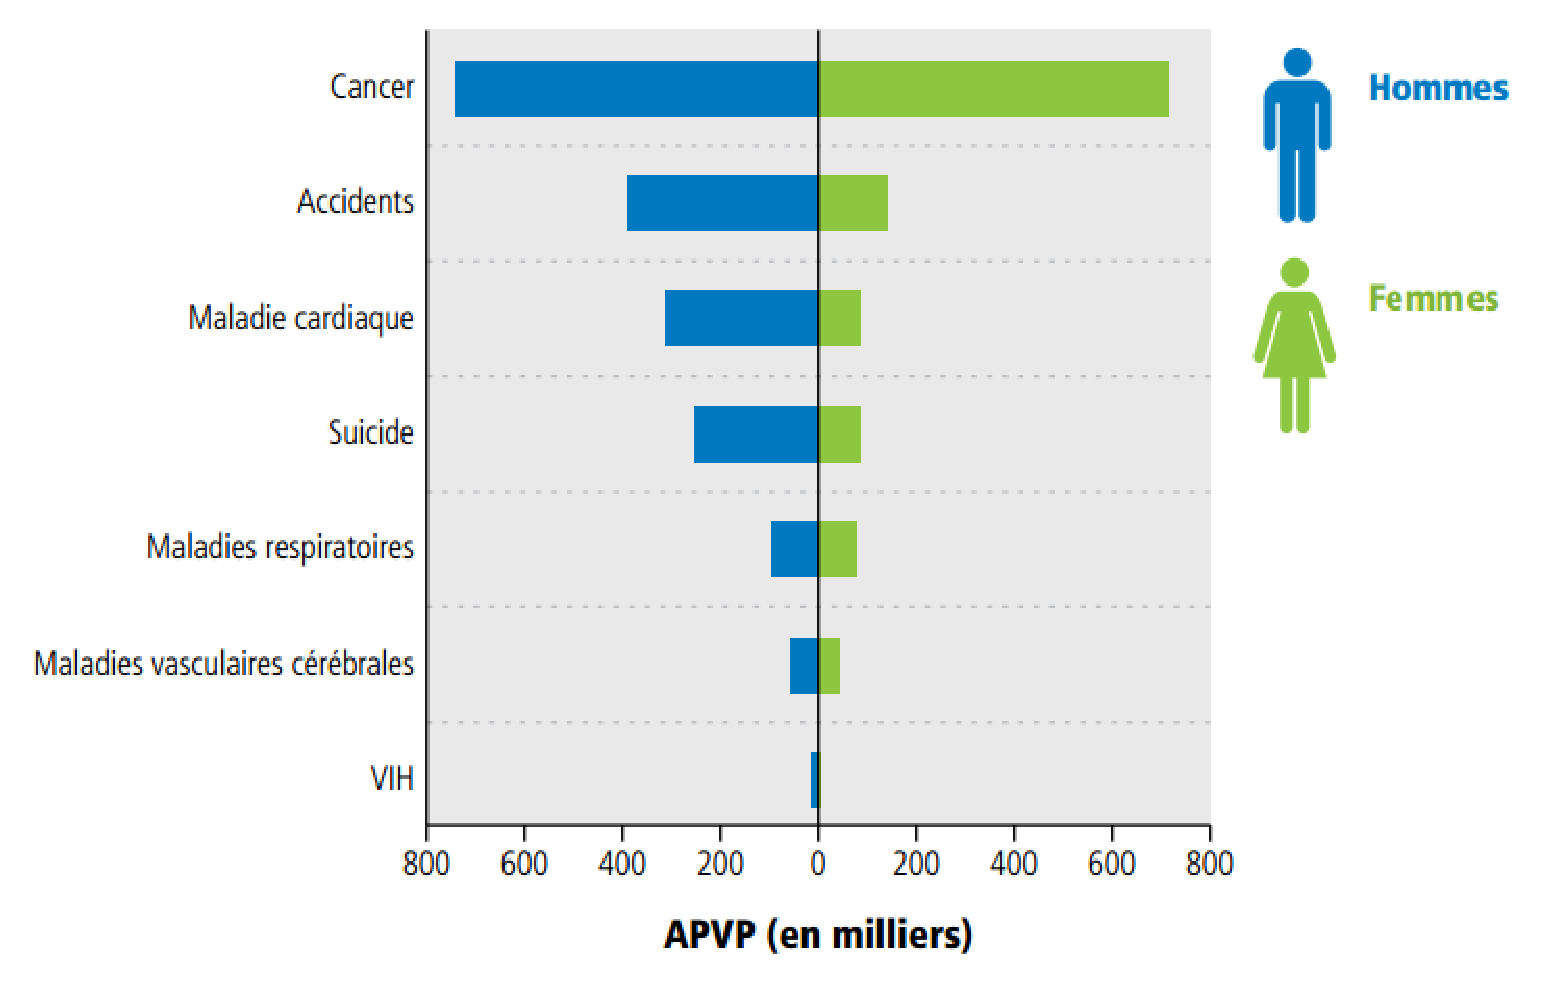
\includegraphics[width=14.0cm,height=9.0cm]{FigureStatCancer2.eps}
\caption{\label{FigureStatCancer2} Années potentielles de vie perdues (APVP) dues au cancer, en comparaison avec les autres causes de décès et leurs distributions selon le sexe. Moyenne des données sur trois ans (2010-2012), Canada, provinces, territoires, régions sociosanitaires et groupes de régions homologues.}
\end{figure}
%
\section{Anatomie et physiologie}
La prostate fait partie du système génital masculin. Chez les jeunes hommes, elle a la taille d’une noix qui augmente progressivement de volume à la fin de la quarante et début de la cinquante. Elle joue un rôle important pour la fertilité de l’homme, notamment, en participant à la formation et la maturation des spermatozoïdes. Elle est responsable de la production d’une grande partie du liquide éjaculé composé du sperme et du liquide prostatique. Sa localisation lui confère également un rôle dans le bon fonctionnement de l'appareil mictionnel, étant donné qu’elle est étroitement liée aux deux sphincters qui assurent une bonne continence urinaire. Comme le montre la figure \ref{FigureProstate} \cite{ImageProstate}, la position de la glande prostatique est dans le petit bassin. Sur sa partie supérieure appelée base, repose la partie inférieure de la vessie, et est localisée en arrière du pubis et devant le rectum. Les organes à risques primordiaux qui compromettent la dosimétrie pour le cancer de la prostate sont la vessie, le rectum et l’urètre dont une partie est contenue dans la prostate (urètre prostatique).
%
\begin{figure}[h]
\centering
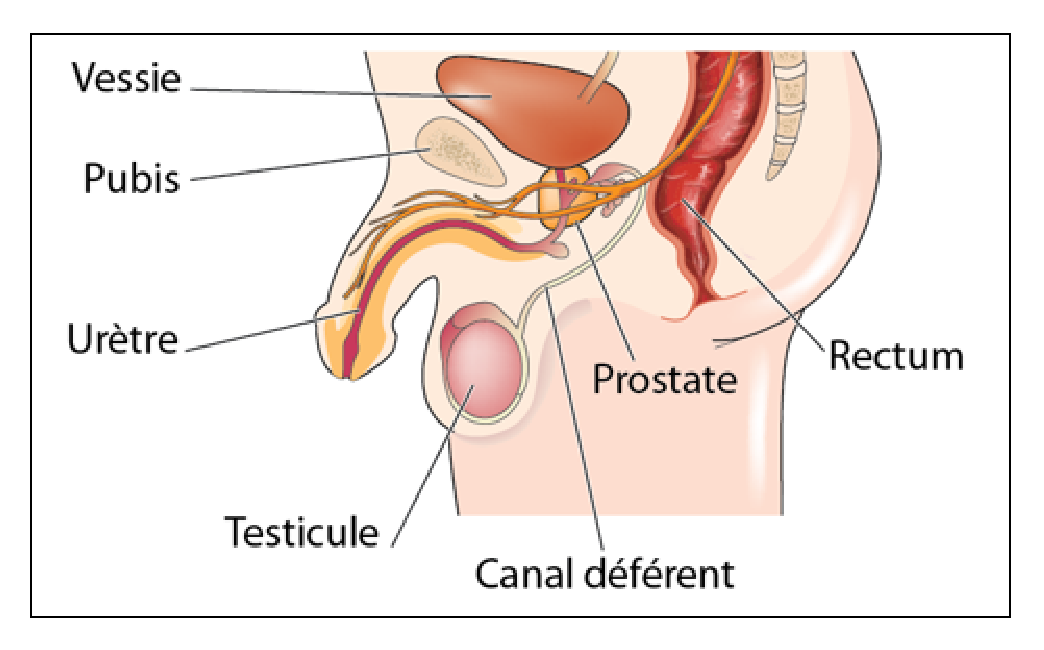
\includegraphics[width=12.0cm,height=8.0cm]{FigureProstate.eps}
\caption{\label{FigureProstate} Anatomie de la prostate et sa localisation par rapport à la vessie et le rectum.}
\end{figure}
\section{Diagnostique}
%
\section{Planicication du traitement en curiethérapie HDR : cas du cancer de la prostate}
%
\subsection{Définition des volumes d'intérêt}
\subsection{Formalisme du calcul de dose: AAPM TG-43}
\nomenclature{AAPM}{American Association of Physicists in Medicine}
%
\subsection{Revue des méthodes d'optimisation}
%
\subsection{Outils d'évaluation d'un plan}
%